%%% Local Variables: 
%%% mode: latex
%%% TeX-master: t
%%% End: 
\documentclass{article}
\usepackage{../tex/mysty}
\begin{document}

\maketitlepage{Societal Impact Report}{Ginger Tsai}

\setcounter{tocdepth}{2}
\tableofcontents
\newpage
\listoftables
\listoffigures
\newpage


\section*{Executive Summary}
\label{sec:exec-summary}

% TODO: Ginger's section


\newpage


\section{Introduction}
\label{sec:introduction}

% TODO: Ginger's section


\section{Notable Concerns}
\label{sec:concerns}

% Introductory sentence (Ginger)


\subsection{Environmental Impact (Joe)}
\label{sec:environment}

The device, being developed for extended use in a controlled setting,
is posed to be highly environmentally conscientious. Due to the
relatively small number of potential buyers, the manufacture,
packaging, and shipping can all be optimized to minimize environmental
impact. The device produces little to no waste during operation and
presents nominal energy draw. Finally, should the device be disposed
of by the end user, it would be easy to reclaim the highly-modular
components for reuse either in new devices or in other projects.

Our proposed manufacturing methods only must serve a small consumer
base of perhaps 300 research labs in the US. At this volume, it is
liable that our devices will be custom fabricated using CNC milling
instead of more volume-dependent manufacturing methods such as
casting. The environmental impact here is that our manufacturing can
operate with a smaller footprint while developing a product that is
more likely to last through more cycles and therefore serve our
consumer base with a minimal environmental offset.

In order to continue with the green methods already proposed, our
device can be packaged in attractive and cheap recycled
materials. Moreover, so long as the device can be user-tested for
designs which are easy and intuitive to use we can easily eschew
providing a printed manual and simply provide that online saving
further packaging mass.

During the lifetime of the device consumes very little material. All
pieces are high quality, robust, and often optically precise requiring
that each component is cleaned and reused instead of being disposed
of. While it is possible that parts such as the mounting cuvet could
shatter if mishandled, care should be taken on the part of the
consumer reducing the frequency of this sort of waste --- after all,
optically-precise cuvets are expensive.

Finally, since the component parts are robust and modular, if a device
does fail it is likely that it can either be easily repaired by a
specialist or recycled to reuse the component parts which are still
operational. Here, the modularity enables us to minimize the impact of
the disposal of damaged, failed devices.

The proposed device therefore is well poised to cause minimal
environmental damage through its manufacture, sale, operation, and
disposal. We support this capability with a commitment to the
environmentally friendly processes available to us by erring on the
side of quality and reusability.


\subsection{Medical Ethics (Joe)}
\label{sec:blah-blah-blah}

As with any research-oriented goal, the distant effects of proximal
successes are difficult to gage; however, since this device most
immediately affects our knowledge of the genetic factors in eye
development --- especially abnormal, myopic eye development --- we can
expect some possibility of discovery there. With any advance in
genetics, there is concern for treatment, identification, and
policy-level decisions concerning those affected by any genetic
predispositions.

For instance, it's foreseeable that the US Air Force, notorious for
rejecting on valid grounds those without 20/20 vision, could extend
their recruitment programs to reject those who have a high chance of
developing myopia (or demanding that they receive elective surgeries
to correct for it). In this case, it's likely a justifiable threat,
but more generally these possibilities can be concerning. The proposed
device could be key in discovering and proving these genetic tests,
and therefore it is important that we consider our part in the
possible development of these policies.

Fortunately, the principal disease being studied is myopia. In the
vast majority of cases there is already a non-invasive, popular
treatment: common eyeglasses. Additionally, as time goes forward it is
likely that our surgical laser-corrective methods will both improve
and drop in price making that an attractive option. Finally, genetic
causes of eye deformation may even be affected \textit{post hoc} by
treating the secondary steps in the development of these diseases. All
of these methods could gain both in awareness, affordability, and
availability from the research enabled by our device.

Even in the worst foreseeable case, should policy fail to prevent
widespread unethical abuse of genetic information, enabling people to
more accurately predict myopia is unlikely to cause much harm. Once
again, there are ample treatment and corrective options available.

To this end, we believe our device to be well in-line with the ethical
principles of today. It's deployment in medical contexts is unlikely
to cause harm to people and instead provide new opportunities to
reclaim ability that normally would be lost to ocular deformation.

\subsection{Sanjay's Blah blah blah}
\label{sec:blah-blah-blah}

\subsection{Sanjay's Blah blah blah}
\label{sec:blah-blah-blah}

\subsection{Shuyen's Demographic}
\label{sec:Demographic}
	The design solution (3D imaging device) is targeted at....
\subsection{Shuyen's Public Policy}
\label{sec:Public Policy}
	The design solution will not be regulated by the FDA ....
\section{Conclusion}
\label{sec:conclusion}

% TODO: Ginger's section

\section{Addendums}
\label{sec:addendums}

\subsection{Tables}
\label{sec:tables}

\begin{table}[H]
  \footnotesize
  \centering
  \begin{tabularx}{\textwidth}{llXX}
    \toprule
    \textbf{Type} & \textbf{Specification} & \textbf{Metric} & \textbf{Justification} \\
    \hline
    Need & Resolution & 2 micron & Choice of scan pattern \\
    Need & Speed & 1 scan within 3 minutes & Choice of scan pattern and drive \\
    Need & 3D image reconstruction & None & Choice of scan pattern \\
    Need & Size & 0.75 by 1m footprint (\textit{or:} fits in 0.75m $\times$ 1m $\times$ 1m space) & Internal compartment design \\
    Need & Electrical Properties & 120V 60Hz AC & Choice of material \\
    Need & Thermal Properties & Functions in $22\pm5$ °C & Choice of material \\
    Need & Chemical Properties & Withstand $<1$ mL of PBS & Choice of material \\
    Need & Robustness & Withstand a drop of 3 feet, sudden sideways movement & Internal compartment design, choice of material \\
    Want & Weight & $<40$ lbs (18 kg) & Internal compartment design, choice of material \\
    Want & User Interface & Requires 1 click of the mouse for measurement transfer from device to computer & Software design \\
    Want & Reusable & Up to 4 years given use of $5^+$ times/day, 1 hour per use & Internal compartment design, choice of material \\
    Want & Minimize vibration & N/A & Component properties \\
    Want & Simplicity & Few hanging, external components; manageable design & External design \\
    Want & Cost & Manufacturing cost $<\$10,000$ & Internal and external design, choice of material \\
    Desire & Aesthetics & Aesthetically pleasing, easy on the eyes & External design, choice of material \\
    Desire & Noise & $<80$ dB & Internal compartment design, choice of material \\
    \bottomrule
  \end{tabularx}
  \figcaption{
    \textbf{Engineering Design Specifications:}
  This is the detailed list of engineering design specifications, categorized by priority in terms of ``need'', ``want'', or ``desire''.}
  \label{tab:eds}
\end{table}

\begin{table}[H]
  \footnotesize
  \centering
  \begin{tabularx}{\textwidth}{XcXX}
    \toprule
    \textbf{Item} & \textbf{Price} & \textbf{Function} & \textbf{Supplier} \\
    \hline
    Keyence LED micrometer                                          & ---      & obtains measurements of eye dimensions                            & adviser - Dr John Nickerson                    \\
    LabVIEW Development System 8.6                                  & ---      & reconstructs and interprets data from micrometer                  & Georgia Tech Biomedical Engineering department \\
    Stanley GR10 Mini Hot Melt Glue Gun                             & \$3.99   & simulates optic nerve                                             & Sears                                          \\
    Stanley 12-Pack All purpose-4" Clear Miniature Glue Sticks      & \$2.00   & simulates optic nerve (in conjunction with hot glue gun)          & thehardwarecity.com (online)                   \\
    plastic ABS mold                                                & ---      & simulates an eyeball                                              & Georgia Tech Biomedical Engineering department \\
    Oral-B Mint Ultra Floss, 1 count, 2 pack                        & \$4.00   & simulates optic nerve (with plastic eyeball)                      & Wal-Mart                                       \\
    Koji eyebrow tweezers                                           & ---      & holds simulated eyeball; simulates tweezer action on optic nerve  & group member                                   \\
    Irwin Quick-Grips                                               & ---      & holds and controls tweezers                                       & Georgia Tech Biomedical Engineering department \\
    Rotational motor                                                & ---      & rotates eyeball                                                   & Georgia Tech Biomedical Engineering department \\
    Firgelli Automations 6" stroke 8lbs Force Linear Actuator 12V   & \$75.00  & vertically translates micrometer and micrometer platform          & robotshop.us (online)                          \\
    Linear Encoder                                                  & \$100.00 & determines position of micrometer                                 & online       \\
    Microscope Stage                                                & \$80.00  & serves as platform upon which micrometer will stand               & online                                  \\
    Wiring                                                          & ---      & connects motors and drives to micrometer and clamp/tweezer system & Georgia Tech Biomedical Engineering department \\
    \hline
    \textbf{Total} & \$345 & & \\
    \bottomrule
  \end{tabularx}
  \figcaption{
    \textbf{Budget for Developing the Prototype:}
  Each component of the prototype is listed along with price, function, and supplier. Blank prices indicate that the component is being provided for free. The final price estimate is lower than the actual anticipated cost as the budget doesn't account for contingencies.}
  \label{tab:expenses}
\end{table}

\subsection{Figures}
\label{sec:figures}

\begin{figure}[H]
  \centering
  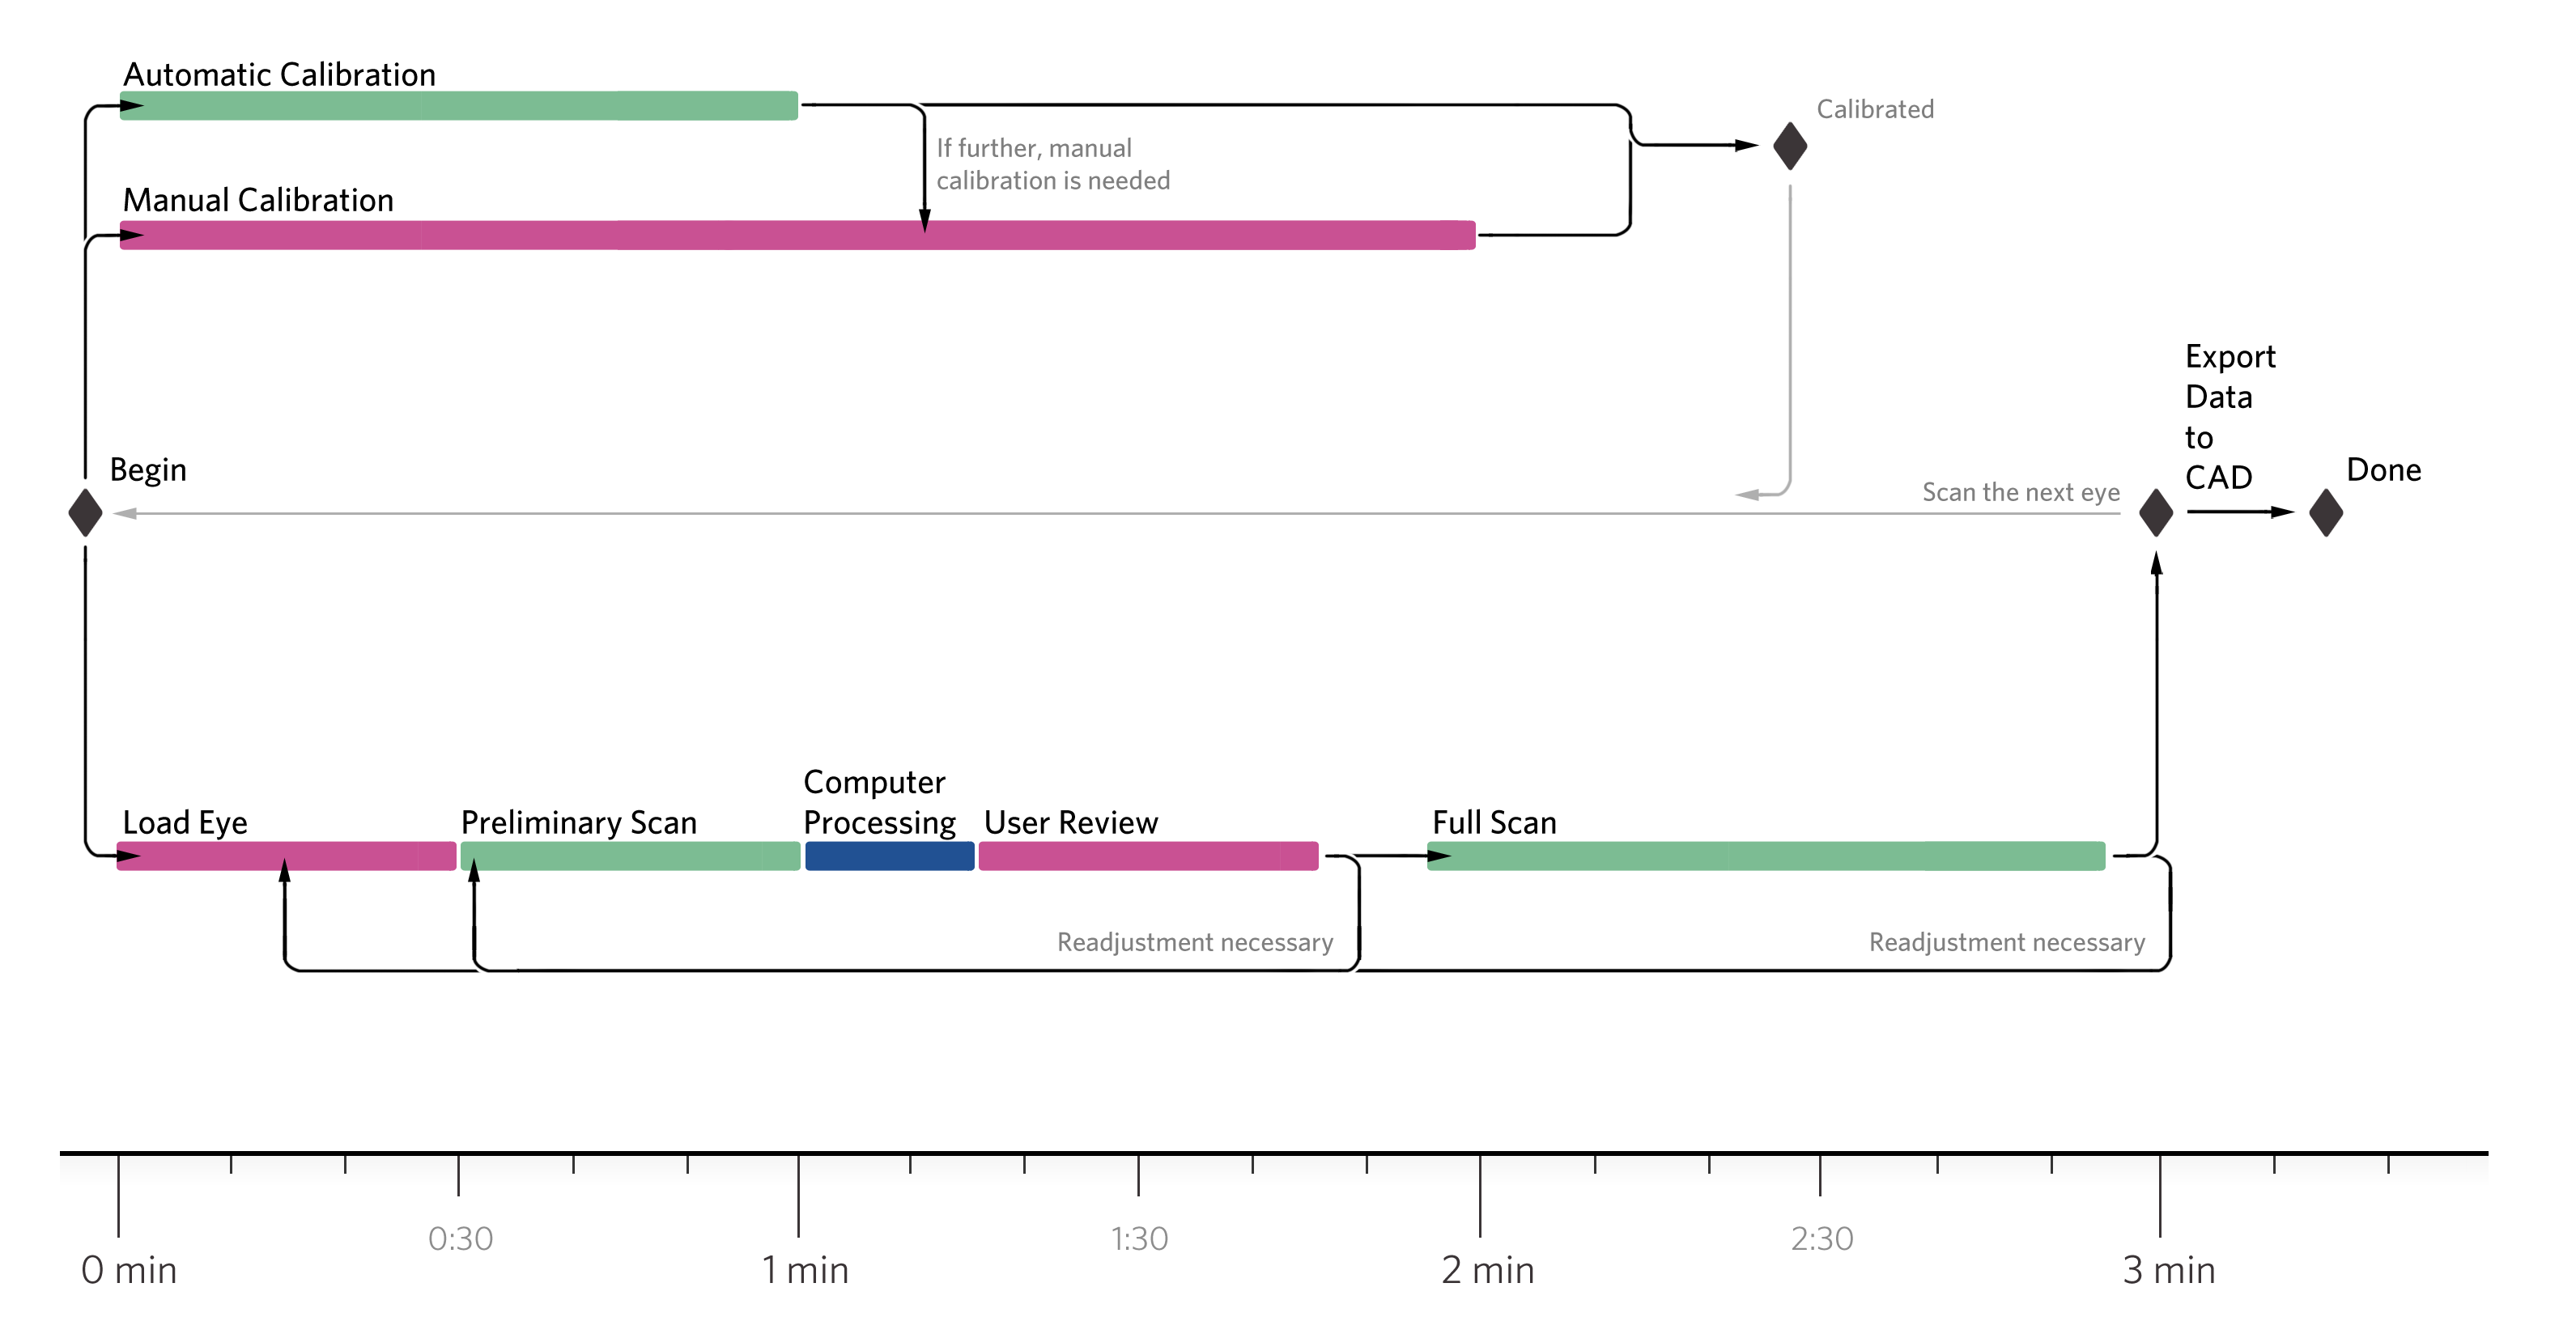
\includegraphics[width=\linewidth]{../img/usage_flow}
  \figcaption{\textbf{Possible Usage Flowchart:}  
  The device is controlled via the computer interface in order to perform a number of tasks required for repeatable, accurate measurement of an eye. Each task is located at and extended over the suggested period of time required to perform the task. Colors of the task boxes encode the required user interaction. Red tasks require direct user interaction with the physical harness, green tasks only require interaction with the computer, and blue tasks are computational tasks where the user must wait.}
  \label{fig:usage}
\end{figure}

\begin{figure}[H]
  \centering
  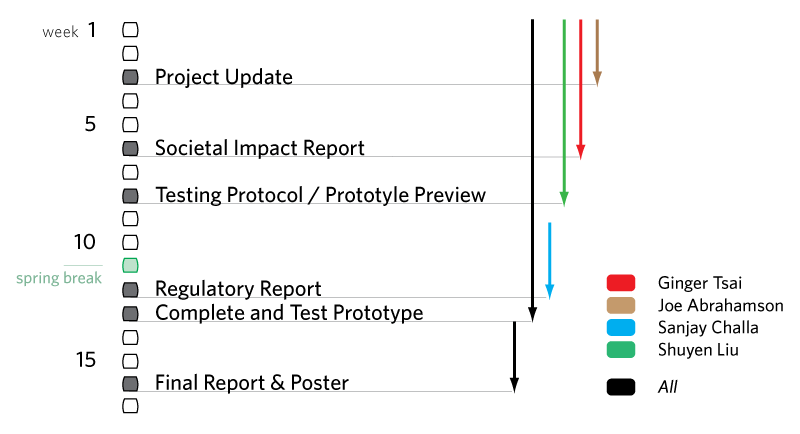
\includegraphics[width=0.75\linewidth]{../img/spring_gantt}
  \figcaption{\textbf{Gantt Chart:}
  The arrows are color coded indicating the primary author of each document. Tasks, duration of tasks, and milestones are clearly illustrated by the arrows and corresponding text at the head of each arrow.}
  \label{fig:gantt}
\end{figure}

\begin{figure}[H]
  \centering
  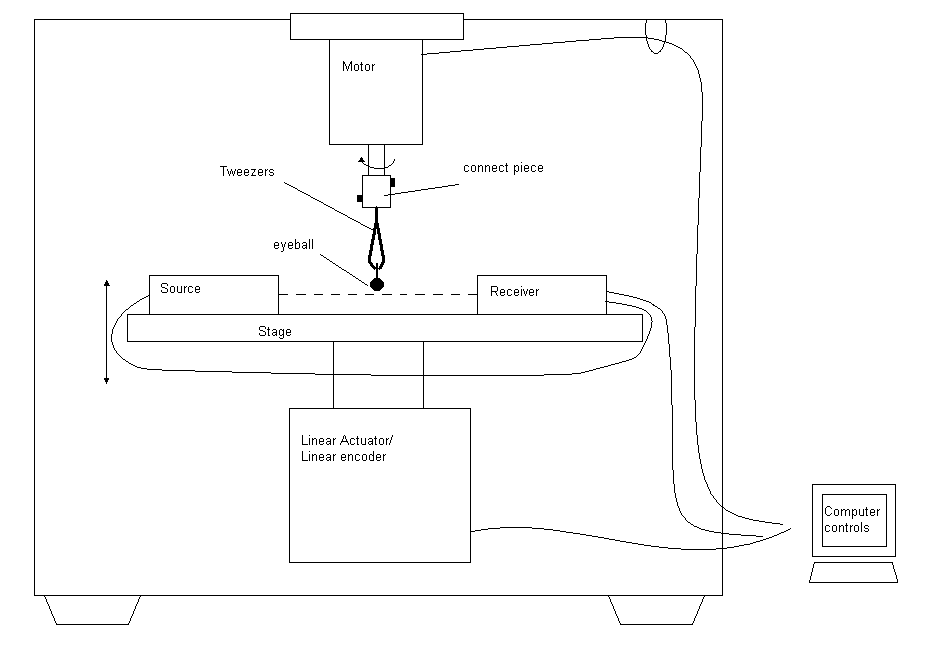
\includegraphics[width=\linewidth]{../img/schematic1}
  \figcaption{\textbf{Schematic of the Prototype:}  
  This figure illustrates the physical organization of the various components of the design within an enclosed framework. Each component is labeled. }
  \label{fig:schematic1}
\end{figure}

\newpage
\addcontentsline{toc}{section}{References}
\bibliographystyle{unsrt}
\bibliography{../tex/bibl}

\end{document}
